Este capítulo apresenta um estudo exploratório realizado com o objetivo de verificar a viabilidade e aperfeiçoar a proposta com base nas descobertas e desafios enfrentados durante o processo. Destaca-se que este estudo teve o foco apenas na análise das avaliações de acessibilidade e não explorou as solicitações de modificações e as alterações realizadas no código das aplicações. 


Todas as decisões de projeto e metodologia adotadas estão em conformidade com o que foi descrito no Capítulo~\ref{chap:proposta}.
Além disso, também são descritas as atividades já realizadas do cronograma proposto.

\section{Questões de pesquisa}

As seguintes questões de pesquisa foram definidas para este estudo exploratório:
\begin{itemize}
 \item RQ1 - Quantas avaliações de usuário são relacionadas à acessibilidade e qual é a sua distribuição? 
 \item RQ2 - Qual é a diversidade de tópicos de acessibilidade abordados nas avaliações dos usuários?
 \item RQ3 - Quais são as notas associadas às avaliações que abordam aspectos de acessibilidade?  
\end{itemize}

\section{Seleção de aplicações móveis}

Os critérios de seleção das aplicações para este estudo seguem os mesmos definidos na Seção~\ref{sec:selecao}. Portanto, foram selecionadas aplicações da plataforma Android que satisfaziam as seguintes condições: estavam disponíveis na \textit{Google Play Store} e o código-fonte se encontrava armazenado em um repositório público da plataforma GitHub. Ao todo, apenas 701 aplicações dentre as mais de 2.000 indexadas no FDroid\footnote{Dados de julho/2019} satisfizeram esses critérios.

A Tabela~\ref{tab:summarygps} mostra a distribuição de alguns atributos das aplicações selecionados por meio de estatística descritiva utilizando o resumo dos cinco números (mínimo amostral, quartil inferior, 
mediana, quartil superior, máximo amostral), a média e o desvio padrão. 
A maioria das aplicações tem até 9 atividades, mas há exemplos muito maiores, como o ``Slide for Reddit'', por exemplo, que possui 91 atividades.

\begin{table}[htb]
%\setlength{\tabcolsep}{0pt}

\centering
\caption{Estatísticas da amostra das avaliações do \textit{Google Play Store}}
\small
\label{tab:summarygps}
\begin{tabular}{lrrrrr}
\hline
             & Atividades & Nota & Avaliações     & Instalações  & Comentários \\
\hline
Mínimo          & 1          & 0     & 0            & 0         & 0       \\
Quartil Inferior           & 2          & 4           & 50    & 1K      & 4       \\
Mediana       & 5          & 4,3   & 130         & 10K     & 22      \\
Quartil Superior          & 9          & 4,6   & 836        & 50K     & 145     \\
Máximo          & 92         & 5     & 3.6M    & 100M & 4.480    \\
Média         & 8,16       & 4,16  & 12.4K     & 550K+    & 305,4   \\
Desvio Padrão        & 10,5       & 0,79  & 151,6K  & 5,7M   & 840,8  \\
\hline
\end{tabular}
\end{table}

A maioria das aplicações possui uma boa nota e foi avaliada por até 836 usuários. O número de avaliações apresentado na tabela é diferente do número de comentários, pois quando um usuário faz uma avaliação ele necessariamente atribui uma nota, mas não é obrigado a inserir um comentário. Existem aplicações que possuem um número muito alto de avaliações, como o Telegram, que possui 3,6 milhões de avaliações. O Telegram também é a aplicação mais instalada (100 milhões de instalações).
Por outro lado, o número de avaliações não é muito alto, visto que a maioria das aplicações recebeu no máximo 145 comentários em suas avaliações. O número máximo de avaliações desta amostra é de 4.480 em razão das limitações da API utilizada. Esta limitação não teve muito impacto neste estudo exploratório porque apenas 15 aplicações (2\%) possuem mais de 4.480 avaliações registradas na \textit{Google Play Store}. 
No momento do estudo piloto, ficou definido que para as novas coletas de avaliações seriam consideradas outras alternativas para que não houvesse limite no número de avaliações retornadas pela API. 


\section{Extração e seleção das avaliações}
\label{sec:extracaoselecao}

Uma aplicação escrita na linguagem Python foi desenvolvida para consumir os dados da \textit{Google Play Store} utilizando a API \emph{google-play-api}\footnote{https://github.com/facundoolano/google-play-api}. Como mencionado anteriormente, na versão utilizada esta API só permitia o retorno de no máximo 4.480 avaliações de cada aplicação. Além disso, só foram recuperadas avaliações escritas em inglês, que é o idioma padrão definido pela API.


A seleção das avaliações que possivelmente estão relacionadas a algum aspecto de acessibilidade da aplicação foi feita por meio da utilização de palavras-chave aplicadas aos comentários dos usuários.
Para isso, um conjunto de palavras-chave foi definido com base nas diretrizes de acessibilidade da BBC~\cite{bbc}, o qual possui 54 recomendações que são classificadas em onze diferentes categorias: áudio e vídeo (5); design (12); editorial (3); foco (6); formulários (6); imagens (2); links (3); notificações (4); scripts e conteúdo dinâmico (4); estrutura (4); e texto equivalente (5). 
Este padrão foi selecionado porque tem o foco em aplicações móveis e possui exemplos de implementação e de teste para cada recomendação, o que permite compreender melhor os tipos de problemas de acessibilidade tratados no guia. 

Foram definidas 213 palavras-chave com base na análise de cada recomendação do guia. 
A Tabela~\ref{tab:keywords} mostra exemplos das palavras-chave utilizadas.
Note que foram consideradas variantes das palavras (exemplo: \textit{cannot see} e \textit{can't see}, ou \textit{color} e \textit{colour}, ou \textit{impaired} e \textit{impairement}) para garantir que nenhuma avaliação relevante fosse excluída. Infelizmente, não é possível capturar casos em que as palavras foram escritas com a grafia errada. A lista completa das palavras-chave pode ser vista em um repositório criado para armazenamento dos dados deste estudo\footnote{https://github.com/marceloeler/data-ihc2019}.


\begin{table}[!htb]
\small
\caption{Exemplos de palavras-chave utilizadas para selecionar avaliações relacionadas à acessibilidade das aplicações}
\label{tab:keywords}
\begin{tabular}{|l|l|}
\hline
Categorias & Palavras-chave \\
\hline
Gerais                    & accessibility, disability, screen reader, Talkback, operable, impaired, 
\\& impairment                                               \\

\hline
Áudio/Vídeo             & subtitle, sign language, audio description,
 transcript, autoplay, mute, \\& volume                                                 \\

\hline
Design                      & contrast, background color, blind, flicker,
 visual cue, touch size, \\&overlap, font size, 
 dark/light mode, eyestrain, seizure, can't see \\

\hline
Editorial                   & consist. label, language, visual/audio cue                                                                \\

\hline
Foco                       & focusable, control focus, keyboard trap, 
 focus order, navigable                        \\

\hline
Formulários                       & unique label, missing label, content description,
 input type, \\& input format, focusable                                                                        \\

\hline
Imagens                      & image of text, hidden text, text alternative,
background image                                                                                               \\

\hline
Links                       & link description, unique desc., duplicate
link, alternative format \\

\hline
Notificações               & inclusive, haptic, vibration, feedback, alert 
 dialog, understandable, \\& unfamiliar                                                                             \\

\hline
Conteúdo dinâmico & animated content, page refresh, automatic  
refresh, timeout,  adaptable, \\&input sign                                                               \\

\hline
Estrutura                   & page title, screen title, heading, header                                                                                                         \\
\hline
Texto equivalente             & alternative text, non-visual, blind, screen reader, content description  \\
\hline
\end{tabular}
\end{table}

O uso de palavras-chave pode trazer muitos falsos positivos, uma vez que várias palavras utilizadas podem ter conotações diferentes de acordo com o contexto. Por isso foi realizada uma análise manual de todas as avaliações que possuíam pelo menos uma palavra-chave definida. Neste estudo, apenas uma pessoa fez a análise manual das avaliações. Além disso, as avaliações não selecionadas por palavras-chave não foram analisadas para saber se alguma delas não foi selecionada pela ausência de alguma palavra-chave relevante e que não foi utilizada. Durante a análise manual, as avaliações confirmadas também foram classificadas em: 
requisições, quando o usuário reporta algum problema de acessibilidade ou solicita alguma modificação ou adição para tornar a aplicação mais acessível;
ou elogios, quando o usuário parabeniza a aplicação pelo seu nível de acessibilidade.


\section{Análise dos resultados}

As avaliações selecionadas com base nas palavras-chave e na validação manual foram analisadas para responder as questões de pesquisa propostas no estudo exploratório. A seguir as respostas às questões de pesquisa são apresentadas em detalhes. 

 
\textbf{RQ1 - Quantas avaliações de usuário são relacionadas à acessibilidade e qual é a sua distribuição? }

No total, foram extraídas 214.053 avaliações completas (com nota e comentário) das 701 aplicações da amostra. 
Dessas avaliações, apenas 5.076 foram pré-selecionadas por meio das palavras-chave. 
Após a análise manual, o número de avaliações relacionadas à acessibilidade das aplicações foi reduzido para 2.663, o que representa apenas 1,24\% de todas as avaliações completas extraídas.

As avaliações de acessibilidade não estão igualmente distribuídas entre as aplicações da amostra.
Só 40\% dos casos (276) possuem pelo menos uma avaliação relacionada à acessibilidade.
É importante ressaltar que 92\% (197.419) de todas as avaliações extraídas foram realizadas para essas 276 aplicações, indicando que quanto menos avaliações, menor são as chances de haver uma avaliação de acessibilidade. 
De fato, a correlação de Spearman calculada entre o número de avaliações e o número de avaliações de acessibilidade é de 0,73, o que representa uma forte correlação.

As avaliações de acessibilidade não estão distribuídas igualmente entre as 276 aplicações.
Quase 65\% das avaliações de acessibilidade (1.745) estão concentradas em apenas 35 aplicações, e dentre essas, três possuem mais de 100 avaliações de acessibilidade enquanto as demais têm entre 19 e 79 avaliações cada. 
A Figura~\ref{fig:distributionreviewsapp} mostra a distribuição de avaliações de acessibilidade entre as aplicações da amostra, com exceção das 35 aplicações mencionadas anteriormente.
É possível perceber que a grande maioria das aplicações têm menos do que nove avaliações de acessibilidade, enquanto cerca de metade da amostra tem até três avaliações do tipo.


\begin{figure}[!htb]
\centering
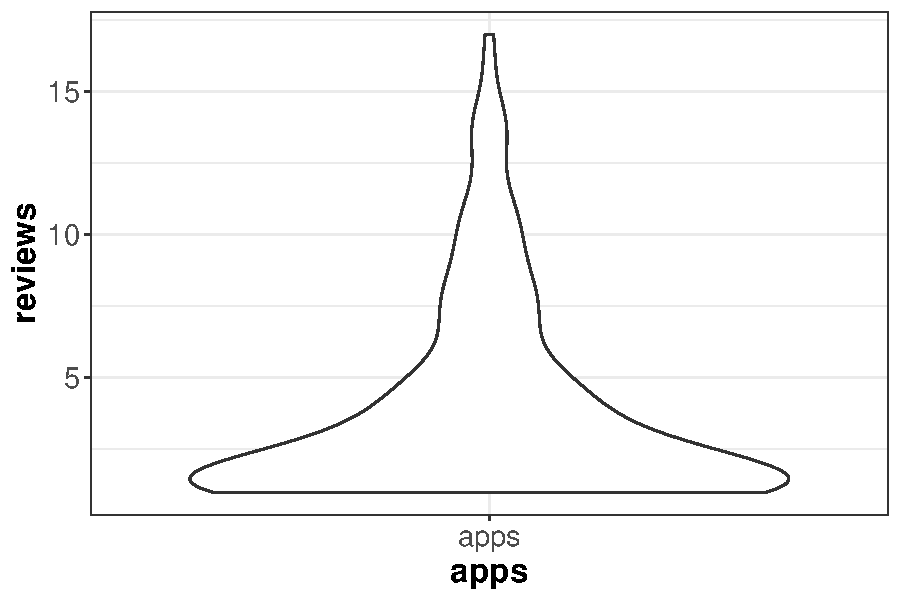
\includegraphics[scale=0.80]{imagens/distribution-accreviews-no-outlier-violin.pdf}
\caption{Distribuição das avaliações de acessibilidade entre as aplicações da amostra}
\label{fig:distributionreviewsapp}
\end{figure}


A Figura~\ref{fig:distribution-proportion} mostra a distribuição da proporção entre as avaliações de acessibilidade e o número total de avaliações completas de cada aplicação.
No geral, as avaliações de acessibilidade representam menos de 4\% de todas as avaliações feitas para cada aplicação, e para metade das aplicações elas representam menos de 1,5\%.
Para uma pequena proporção de aplicações, as avaliações de acessibilidade representam entre 4\% e 9\% do total de avaliações recebidas. Existem algumas aplicações para as quais essa proporção varia entre 10\% e 16\%.
Há alguns casos em que o número de avaliações completas é tão pequeno que uma simples avaliação de acessibilidade representa uma grande proporção, como é o caso das aplicações MuPDF mini, Booky McBookface, e GameDealz, cujas proporções são de 50\% (1/2), 40\% (2/5) e 33\% (1/3), respectivamente. 
\newline 

\begin{figure}[!htb]
\centering
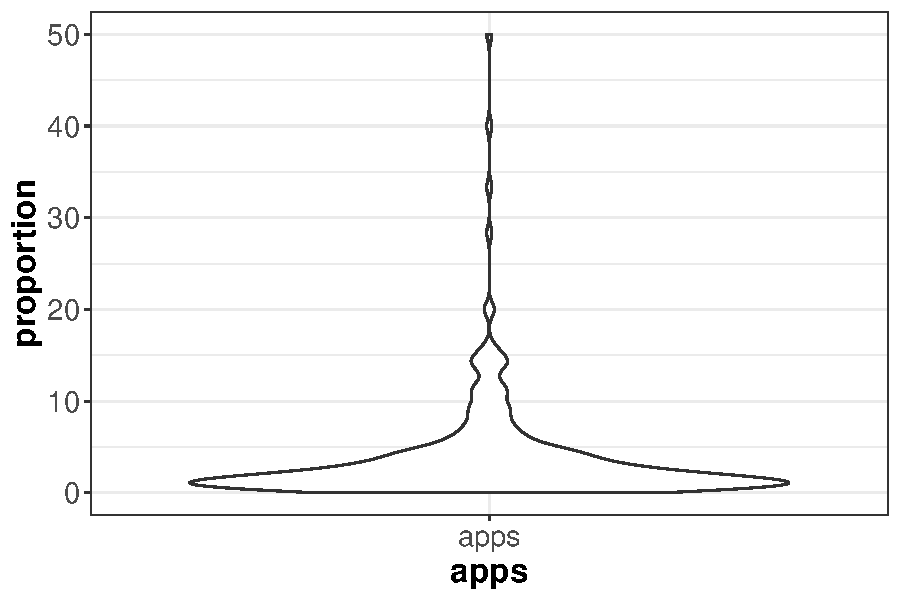
\includegraphics[scale=0.8]{imagens/distribution-proportion-accreviews}
\caption{Distribuição da proporção entre avaliações de acessibilidade e o total de avaliações de cada aplicação}
\label{fig:distribution-proportion}
\end{figure}


\textbf{RQ2 - Qual é a diversidade de tópicos de acessibilidade abordados nas avaliações dos usuários?}

O objetivo desta questão de pesquisa é entender se os usuários abordam diferentes problemas de acessibilidade em suas avaliações ou se a maioria das avaliações trata-se de um conjunto restrito de problemas. 
A Tabela~\ref{tab:keywords-reviews} mostra o número de avaliações de acessibilidade e aplicações associadas a cada palavra-chave utilizada para selecionar as avaliações. 
Nesta tabela só estão apresentadas as palavras-chave para as quais pelo menos uma avaliação estava associada. 

\begin{table*}[!htb]
\centering
\small
\setlength{\tabcolsep}{3pt}
\caption{Número de avaliações e aplicações por palavra-chave}
\label{tab:keywords-reviews}
\begin{tabular}{lrr||lrr||lrr}
\hline
palavra          & avals.  & apps & palavra          & avals.  & apps &  palavra           & avals.  & apps \\
\hline
dark mode        & 645     & 128  & metadata         & 20      & 12   & grouped            & 3       & 3    \\
zoom             & 491     & 80   & too bright       & 20      & 8    & seizures           & 3       & 1    \\
customization    & 309     & 50   & haptic           & 16      & 10   & select language    & 3       & 3    \\
font size        & 214     & 74   & scaling          & 16      & 11   & understandable     & 3       & 3    \\
volume           & 146     & 40   & control key      & 15      & 5    & vibration feedback & 3       & 3    \\
cannot see       & 128     & 57   & voice command    & 14      & 10   & actionable         & 2       & 1    \\
accessibility    & 74      & 44   & text-to-speech   & 13      & 9    & audio cue          & 2       & 2    \\
readable         & 72      & 47   & eyestrain        & 12      & 9    & missing label      & 2       & 2    \\
change font      & 68      & 44   & strain           & 12      & 9    & navigable          & 2       & 2    \\
hard to see      & 58      & 41   & backgrd. image   & 11      & 8    & verbose            & 2       & 2    \\
backgrd. color   & 50      & 30   & screen reader    & 11      & 10   & captcha            & 2       & 2    \\
light mode       & 42      & 27   & change language  & 10      & 8    & audio description  & 1       & 1    \\
mute             & 42      & 25   & small widget     & 10      & 9    & container          & 1       & 1    \\
contrast         & 40      & 31   & stop button      & 10      & 5    & distinguishable    & 1       & 1    \\
subtitle         & 40      & 7    & impaired         & 9       & 9    & input type         & 1       & 1    \\
adjustable       & 34      & 23   & text reflow      & 9       & 3    & keyboard language  & 1       & 1    \\
blind            & 31      & 24   & timeout          & 9       & 7    & page refresh       & 1       & 1    \\
header           & 31      & 22   & consistency      & 7       & 7    & page title         & 1       & 1    \\
overlap          & 31      & 25   & epilepsy         & 7       & 1    & sign language      & 1       & 1    \\
pause button     & 27      & 17   & assistance       & 6       & 5    & svg image          & 1       & 1    \\
flicker          & 26      & 19   & colour coding    & 5       & 5    & switch device      & 1       & 1    \\
spacing          & 26      & 17   & transcript       & 5       & 5    & touch target       & 1       & 1    \\
migraine         & 25      & 3    & default language & 4       & 4    & adjust size        & 1       & 1    \\
input method     & 23      & 11   & older device     & 4       & 3    & adjust colour      & 1       & 1    \\
autoplay         & 21      & 17   & visual cue       & 4       & 4    &                    &         &     \\
\hline
\end{tabular}
\end{table*}

Claramente, as avaliações de acessibilidade estão concentradas em um pequeno conjunto de palavras-chave. Seis das palavras-chave mais populares são mencionadas em mais de 100 avaliações de diferentes aplicações. Por exemplo, a palavra-chave \textit{dark mode} aparece em 628 avaliações de 128 aplicações distintas, o que representa quase metade da amostra de aplicações.

Como várias palavras-chave podem estar relacionadas a uma mesma diretriz ou princípio de acessibilidade (exemplo: \textit{dark mode}, \textit{night mode} e \textit{black mode}), 
as palavras-chave e as respectivas quantidades de avaliações foram agrupadas por tópicos (diretrizes, princípios ou temas) específicos de acessibilidade para facilitar a análise da diversidade de características abordadas.

A Tabela~\ref{tab:group-keywords} mostra, para cada tópico de acessibilidade (Coluna 1), o número de avaliações distintas (Coluna 2), a proporção das avaliações em relação às avaliações de acessibilidade (Coluna 3), o número de aplicações distintas que tiveram uma avaliação relacionada (Coluna 4), e a proporção de aplicações que possuem pelo menos uma avaliação (Coluna 5).
As diretrizes gerais da BBC não foram utilizadas para a organização dos tópicos apresentados na tabela porque eles são muito gerais e podem englobar muitas palavras-chave ao mesmo tempo.

\begin{table}[]
\centering
\caption{Distribuição de avaliações de acessibilidade e aplicações por tópico de acessibilidade}
\label{tab:group-keywords}
\begin{tabular}{lrrrr}
\hline
Tópico        & Avals.  & \% (Avals.) & Apps & \% (Apps) \\
\hline
Theme/Mode    & 726     & 27\%        & 144  & 52\%  \\
Zoom          & 506     & 19,0\%      & 83   & 30,1\%  \\
Customization & 351     & 13\%        & 63   & 23\%  \\
Media         & 309     & 11,6\%      & 82   & 29,7\%  \\
Font          & 249     & 9,4\%       & 83   & 30,1\%  \\
Contrast      & 218     & 8\%         & 91  & 33\%  \\
Impairment    & 135     & 5,1\%       & 70   & 25,4\%  \\
Flickering    & 87      & 3,3\%       & 31   & 11,2\%  \\
Accessibility & 74      & 2,8\%       & 44   & 15,9\%  \\
Size          & 66      & 2,5\%       & 45   & 16,3\%  \\
Input alternatives        & 54       & 2,0\%      & 25   & 9,1\%   \\
Feedback      & 19      & 0,7\%      & 11   & 4,0\%   \\
Language      & 15      & 0,6\%      & 11   & 4,0\%  \\
\hline
\end{tabular}
\end{table}

O tópico \textit{Theme/Mode} é o mais popular entre as avaliações uma vez que 27\% das avaliações de acessibilidade estão relacionadas a este tópico, e quase metade das aplicações tem este tipo de avaliação. 
Este tópico agrega todas as avaliações que mencionam modos de cores e temas das interfaces das aplicações. 
O segundo tópico mais popular é o relacionado a funcionalidades de \textit{zoom} (19\% das avaliações de acessibilidade e 30\% das aplicações).
O terceiro tópico mais popular está relacionado à personalização da aplicação, representando 13\% das avaliações e relacionados a 23\% das aplicações. 
Diversos outros tópicos estão presentes em um número menor de avaliações de acessibilidade, mas muitos deles estão relacionados com um grande número de aplicações. 

Além da análise de todas as avaliações em conjunto, também foram realizadas análises das diversidades de tópicos de acessibilidade de cada aplicação isoladamente. 
Figura~\ref{fig:distributiontopicsapps} mostra a distribuição de palavras-chave encontradas nas avaliações de acessibilidade de cada aplicação (lado esquerdo). 
No geral, há pouca diversidade de palavras-chave nas avaliações de cada aplicação analisada individualmente. 
A correlação de Spearman entre a diversidade de palavras-chave e o número de avaliações em cada aplicação é de 0,93, o que indica que a diversidade aumenta conforme aumenta o número de avaliações.


\begin{figure}[!htb]
\centering
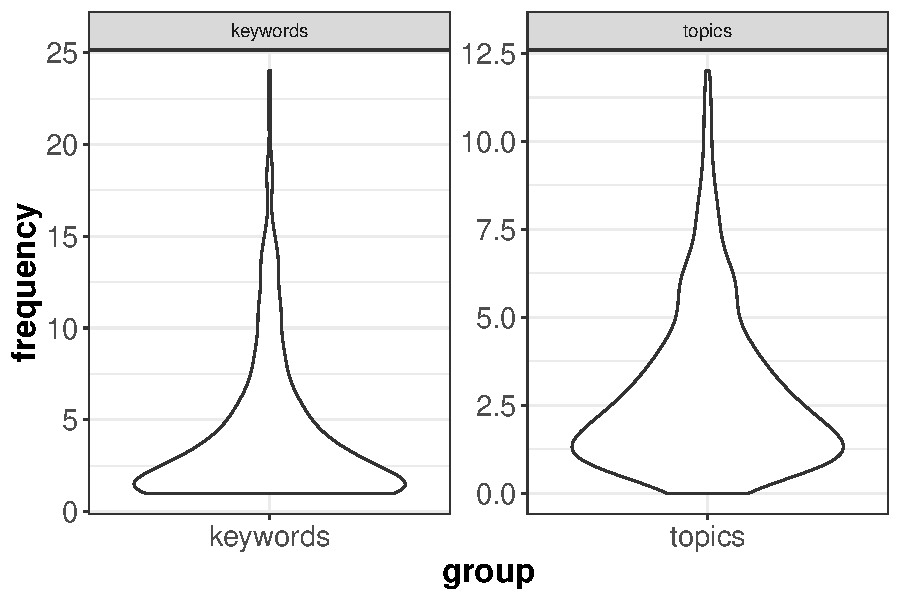
\includegraphics[scale=0.8]{imagens/distribution-topics-keywords.pdf}
\caption{Distribuição de tópicos de acessibilidade e palavras-chave nas avaliações de cada aplicação}
\label{fig:distributiontopicsapps}
\end{figure}


Para a maioria das aplicações, as avaliações de acessibilidade estão relacionadas a no máximo seis palavras-chave. 
Para metade das aplicações, no máximo três palavras-chave são mencionadas. 
Poucas aplicações têm avaliações que mencionam mais de 15 palavras-chave. 
Uma das aplicações que foge ao padrão é o \textit{Cool Reader}, pois em suas avaliações foram encontradas 36 palavras-chave distintas. 


A diversidade de palavras-chave não é uma indicação de que diversos aspectos de acessibilidade são tratados uma vez que muitas delas estão relacionadas a um mesmo problema, e por isso uma análise por tópico deve ser realizada. 
A Figura~\ref{fig:distributiontopicsapps} mostra a distribuição de tópicos de acessibilidade relacionados a cada avaliação de acessibilidade (lado direito). 
Note que as avaliações de acessibilidade para a maioria das aplicações estão concentradas entre dois e quatro tópicos, enquanto algumas aplicações possuem avaliações associadas a quase todos os tópicos abordados. 
A aplicação \textit{Calculator}, por exemplo, tem avaliações de acessibilidade que abordam 12 tópicos de acessibilidade distintos. 
Embora a correlação de Spearman entre a diversidade de tópicos e o número de avaliações seja de 0,87, o que representa uma correlação forte, esta aplicação possui apenas 60 avaliações. \newline


\textbf{RQ3 - Quais são as notas associadas às avaliações que abordam aspectos de acessibilidade?}


Durante a validação manual (ver Seção~\ref{sec:extracaoselecao}), as avaliações foram classificadas entre requisições (76\%) ou elogios (24\%).
As 645 avaliações que elogiam a acessibilidade estão distribuídas por 110 aplicações, enquanto as requisições estão distribuídas por 262 aplicações. 
Um dos propósitos desta questão de pesquisa é entender se os usuários dão uma nota boa para a aplicação quando fazem um elogio e uma nota ruim quanto fazem alguma requisição. 
A Figura~\ref{fig:reqcompscores} mostra a comparação das notas recebidas pelas avaliações classificadas nessas duas categorias. Aparentemente, não há nenhuma diferença significativa entre as notas atribuídas aos dois grupos.

\begin{figure}[!htb]
\centering
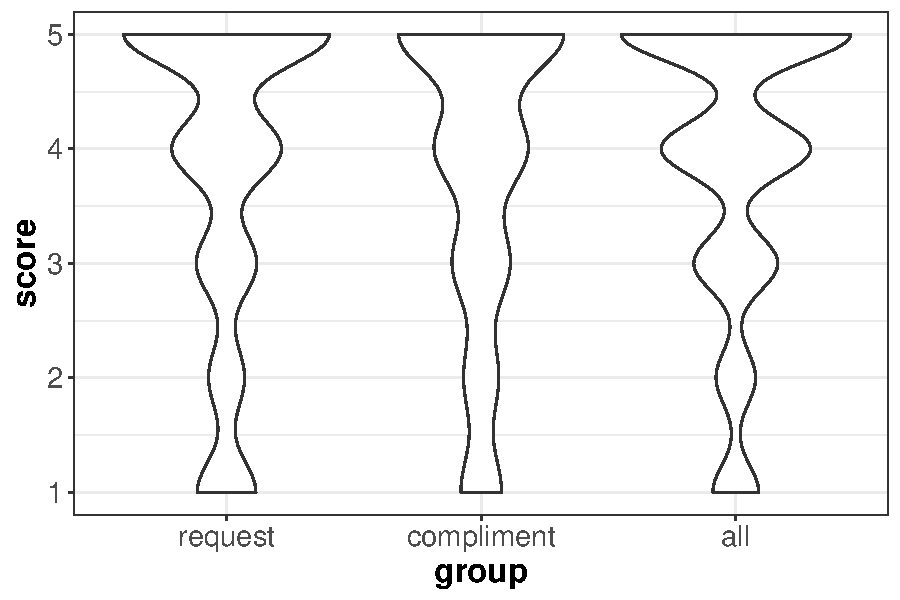
\includegraphics[scale=0.8]{imagens/scores-compliment-request.pdf}
\caption{Comparação entre as notas associadas a avaliações que contém requisições com as avaliações que contém elogios à acessibilidade das aplicações}
\label{fig:reqcompscores}
\end{figure}

Adicionalmente, deseja-se descobrir se avaliações associadas a diferentes palavras-chave ou tópicos de acessibilidade possuem notas maiores ou menores. 
A Figura~\ref{fig:scoresthemes} mostra as notas associadas a cada tópico de acessibilidade (ver Tabela~\ref{tab:group-keywords}). 
Neste caso, somente foram consideradas avaliações que contém requisições. 
Para alguns tópicos específicos, mesmo que haja requisição dos usuários para tornar as aplicações mais acessíveis, as notas são, em sua maioria, 4 ou 5 (exemplo: \textit{customization}, \textit{font}, \textit{media}, \textit{size} e \textit{theme}).
Para outros tópicos, entretanto, as notas estão concentradas em valores mais baixos, de 2 a 4 (exemplo: \textit{contrast}, \textit{flickering} e \textit{zoom}). 


\begin{figure}[!htb]
\centering
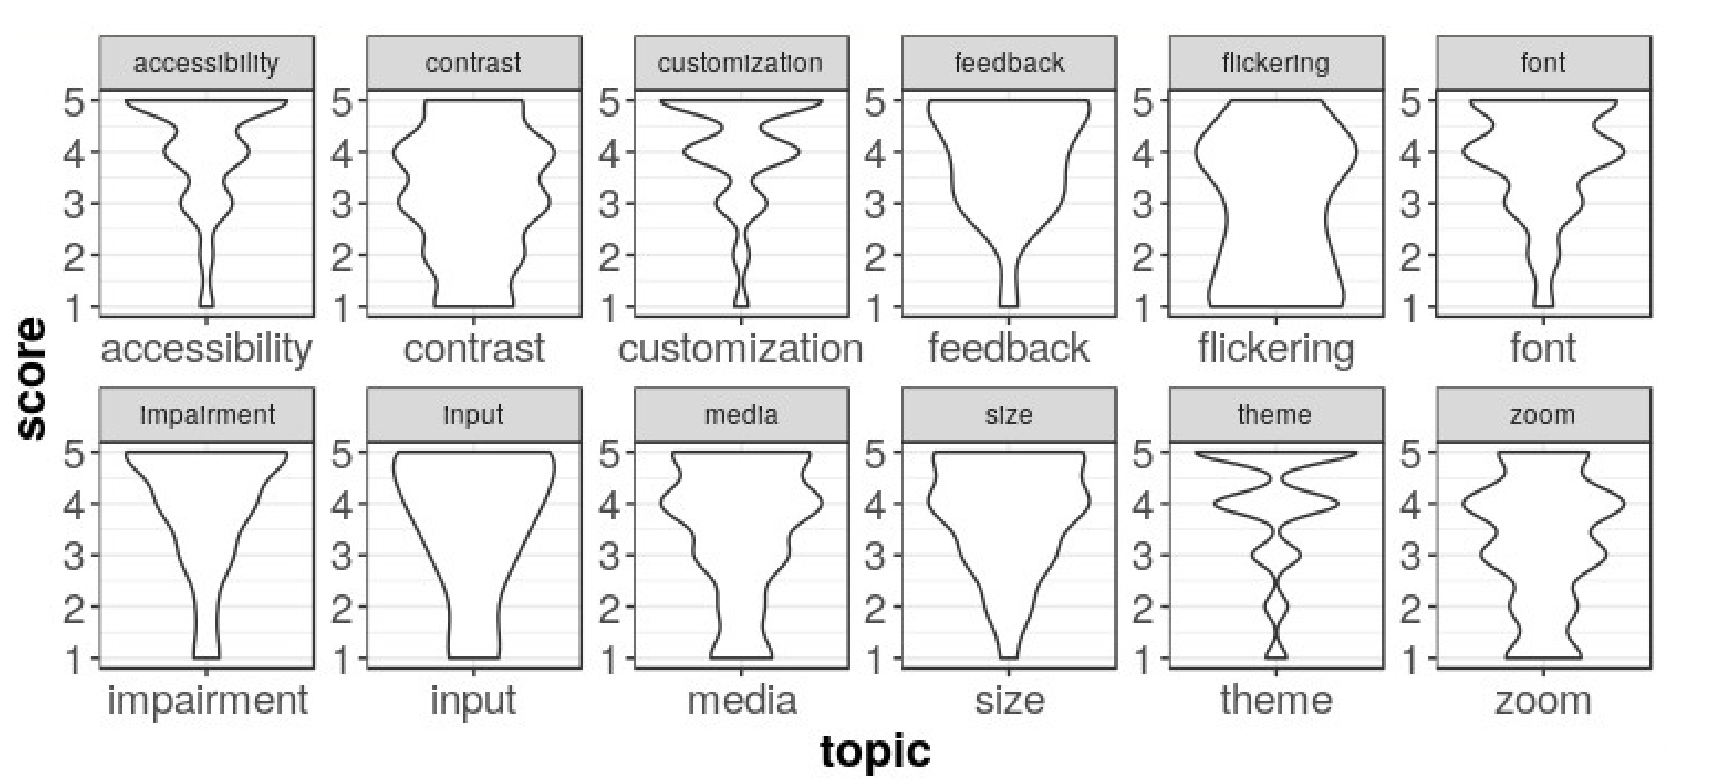
\includegraphics[scale=0.57]{imagens/score-themes-adapt.pdf}
\caption{Notas associadas às avaliações que abordam um tópico de acessibilidade (cf. \autoref{tab:group-keywords})}
\label{fig:scoresthemes}
\end{figure}

A Figura~\ref{fig:scoreskeys} mostra as notas associadas a avaliações que contém algumas das palavras-chave utilizadas neste estudo. 
Para algumas palavras-chave as notas estão concentradas nos valores máximos (\textit{accessibility}, \textit{blind}, \textit{change font}, \textit{dark mode}, \textit{customization}, \textit{haptic}, etc), para outras palavras-chave as notas são significativamente mais baixas (\textit{cannot see}, \textit{epilepsy}, \textit{flicker}, \textit{migraine}, \textit{readable}, \textit{text reflow} e \textit{too bright}). 

\begin{figure}[!htb]
\centering
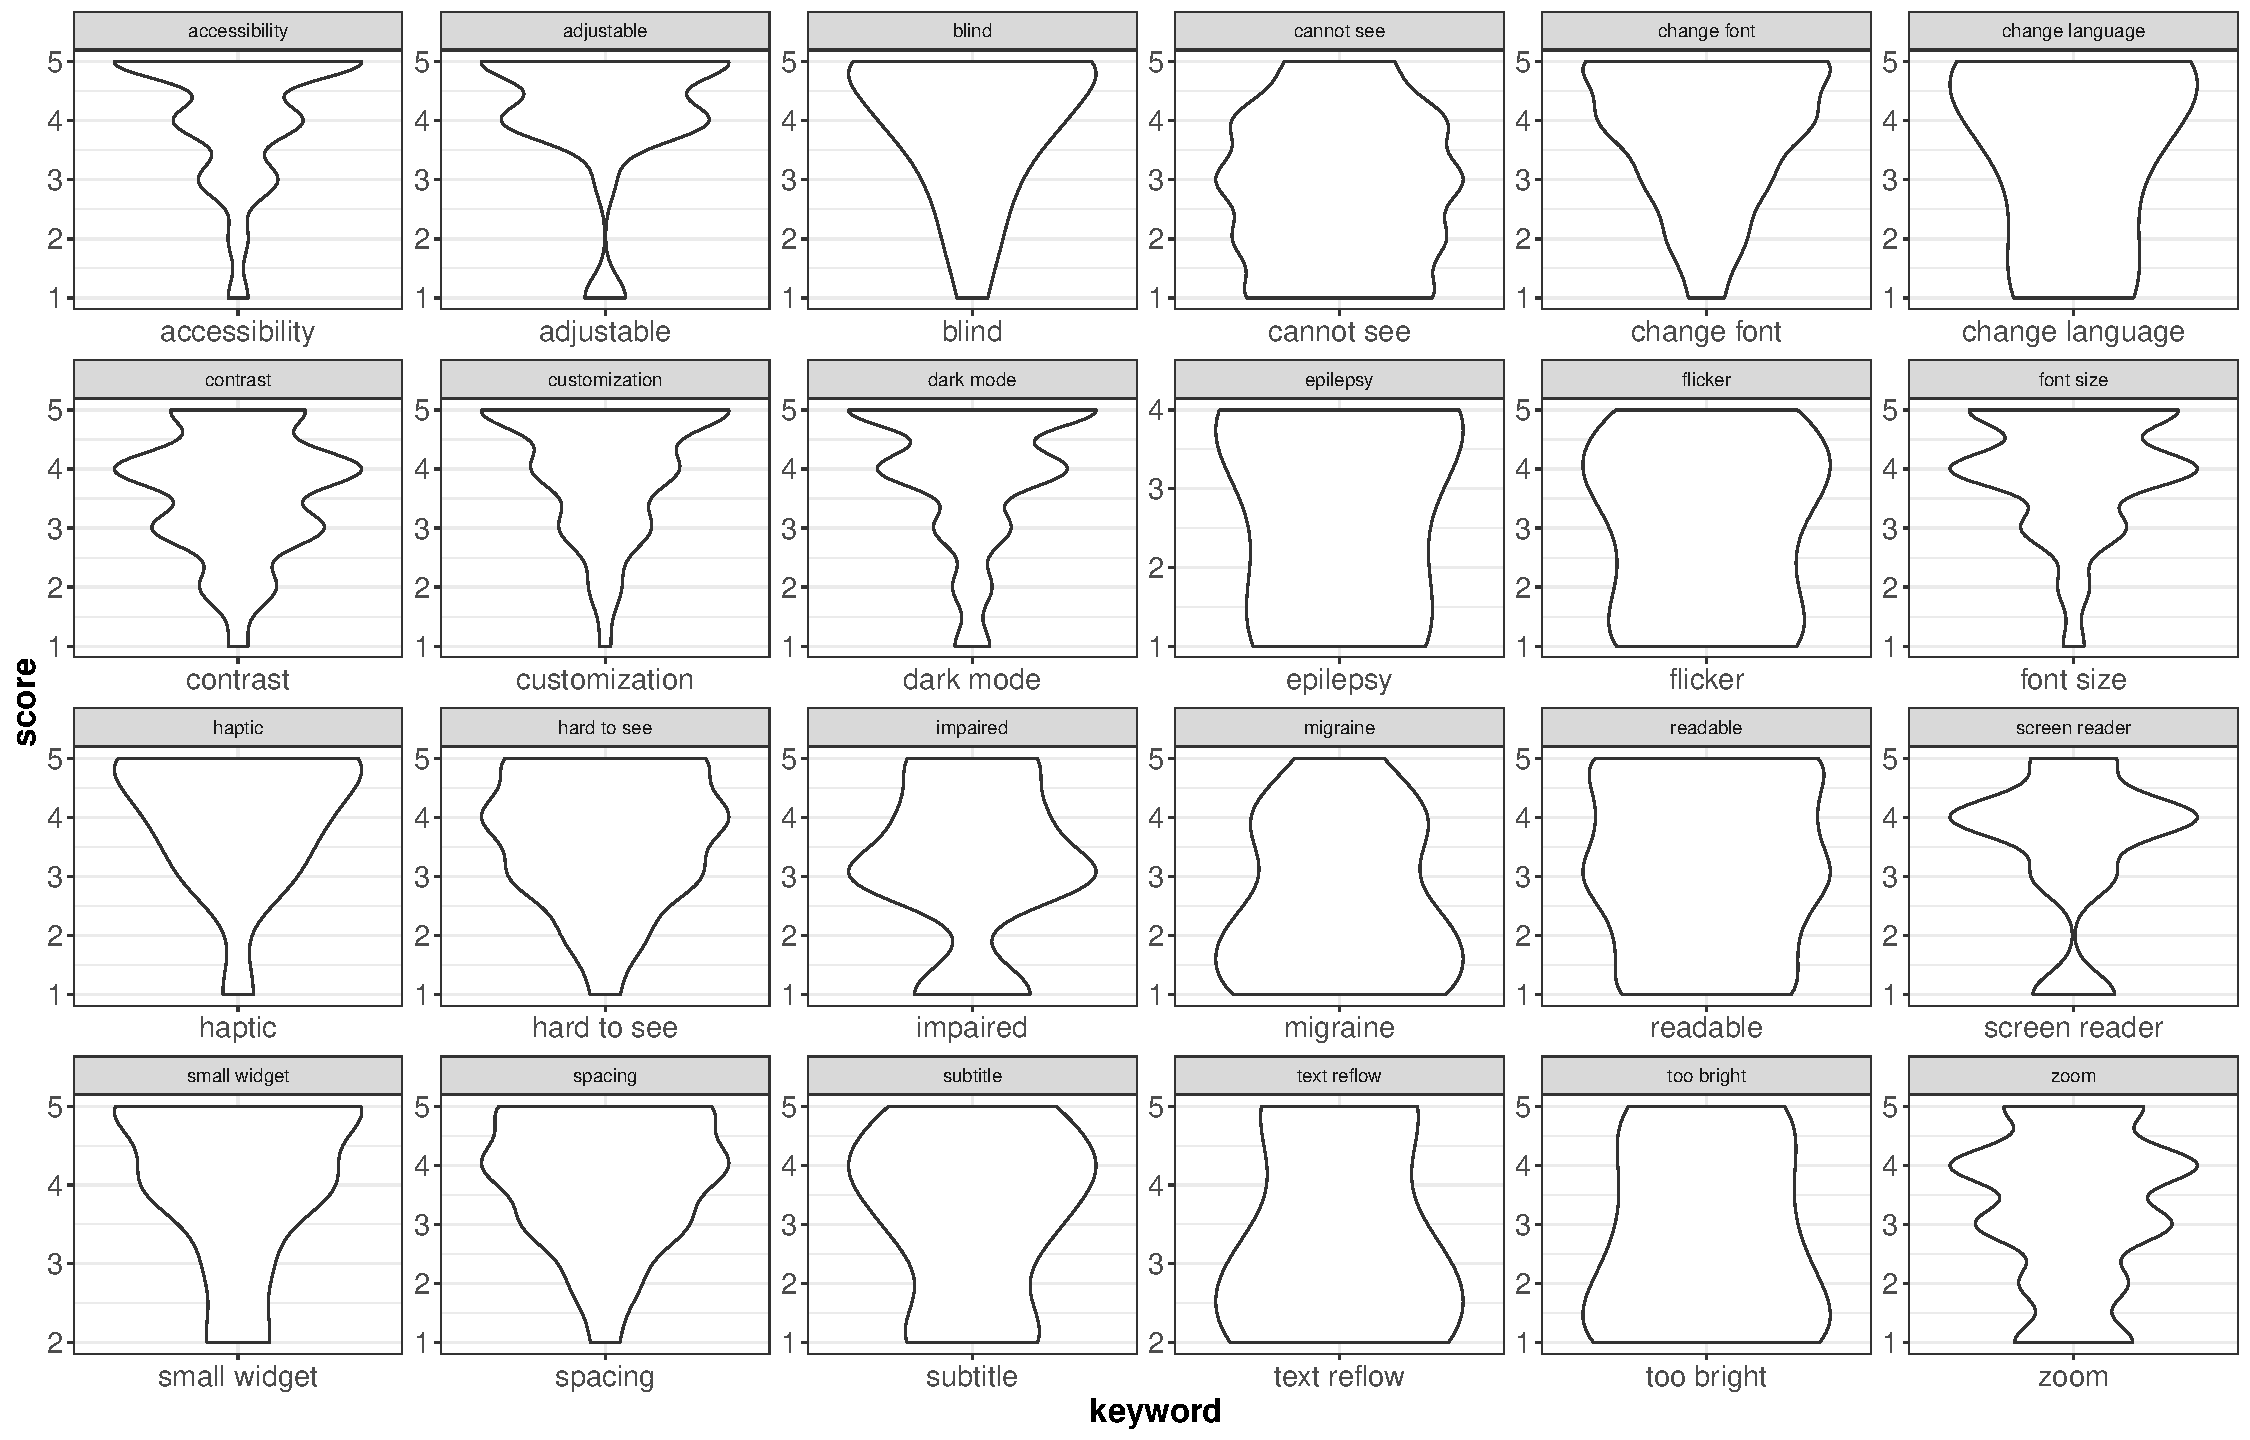
\includegraphics[scale=0.42]{imagens/keywords-scores.pdf}
\caption{Notas associadas aos comentários que apresentam uma determinada palavra-chave}
\label{fig:scoreskeys}
\end{figure}

Aparentemente, os usuários só atribuem notas baixas às aplicações quando encontram problemas de acessibilidade que são barreiras para a utilização da aplicação. 
Alguns exemplos de comentários de usuários encontrados nas avaliações que contém palavras-chave associadas às menores notas estão apresentados a seguir:
\begin{itemize}
 \item \textit{``Very little contrast. Bad for old eyes.''}
 \item \textit{``Wish it also handled older open doc formats - and that it would reflow text on zoom''}
 \item \textit{`` The flashing backgrounds could trigger an epilepsy and migraine''}
 \item \textit{``It's ok but the editing icons come up in white over the image.. which obviously means if you have a white image you cannot see them. Seriously - how could a developer get something so obvious that wrong? ''}
 \item \textit{`` Widget Text color is black. Unreadable''}
 \item \textit{``Too bright now on this update now. Can you option to inverted color? (black instead of white). Going to have to uninstall. Sorry.''}  
\end{itemize}



\section{Discussão}

A maioria das avaliações de acessibilidade encontradas foram feitas por usuários que não necessariamente estavam tratando diretamente da acessibilidade da aplicação. Ainda que essas avaliações mencionem aspectos da aplicação que influenciam a sua acessibilidade, nem todas elas são requisições relacionadas a barreiras encontradas pelos usuários, mas solicitações para melhorar sua experiência de uso. 
Embora poucos usuários se identifiquem como pessoas com deficiência em suas avaliações, percebe-se que as requisições realizadas por eles são associadas a barreiras reais encontradas durante o uso da aplicação, acompanhadas de notas mais baixas. 

Em geral, pessoas com deficiência tendem a ser enfáticas sobre as barreiras que as impedem de usar plenamente a aplicação. A seguir são apresentados alguns exemplos de comentários feitos por pessoas com deficiência:
\begin{itemize}
 \item \textit{``I am legally blind and use Voice Assistant. This app does not interface well with Voice Assistant. It jumps to reading the logo - when trying to get to next group or text to be read. Extremely frustrating! Please fix right away!''}
  \item \textit{``The layout of the app is miserable for those with visual impairments. Please rethink your layout for those who can't read the tiny clues (even on a tablet!)''}
  \item \textit{``Some buttons are unlabelled (I've figured out which ones are repeat and shuffle - I still don't think I know what some are). Also the sleep timer is half-way accessible - when I was using the slider to select the minutes it wouldn't read the amount of time I selected (might be the fault of the screen reader though - I'm using the Mobile Accessibility screen reader from Code Factory).''}
  \item \textit{``Hello. If this app become accessible to Talkback (android screen reader) I wish the best for you developers. Actually we blinds can use telegram only on ios because it is accessible with Voiceover (IOS screen reader). One of my friends needs it because he does not have money to buy an apple product but he has a cheap android device and he needs telegram on it because of their university channel on telegram. If this app becomes accessible I will rate it 5 or more!''}
  \item \textit{``What are you trying to do? Give someone who has epilepsy a seizure? I almost did. Thanks a lot, idiots''}  
\end{itemize}

A escassez e a homogeneidade das avaliações de acessibilidade associadas às boas notas recebidas em geral pelas aplicações parece indicar que ou os usuários com deficiência não utilizam essas aplicações ou eles tendem a não realizar avaliações. 
Nos estudos ampliados que serão realizados com base neste estudo exploratório, pretende-se fazer análise separadas de avaliações que claramente foram escritas por pessoas com alguma deficiência ou que enfrentaram uma barreira real para a utilização da aplicação pela falta de acessibilidade. 

Por fim, considerando que as avaliações dos usuários são uma poderosa ferramenta para guiar a evolução de aplicações móveis~\cite{Iacob2014online,Panichella2015how,Palomba2018crowdsourcing}, 
esses resultados preliminares sugerem que isso não tem sido utilizado apropriadamente para pressionar desenvolvedores e organizações na melhoria da acessibilidade das aplicações.

\section{Publicações}
\label{sec:publicacoes}

Os resultados deste estudo exploratório foram divulgados em artigo completo publicado na trilha principal do XVIII Simpósio Brasileiro sobre Fatores Humanos em Sistemas Computacionais (IHC 2019)~\cite{ihc2019}. Destaca-se que este artigo recebeu o prêmio de melhor artigo do IHC 2019. 

\section{Novas configurações de estudo e atividades realizadas}
\label{sec:atividadesrealizadas}

O planejamento e os resultados do estudo apresentado anteriormente foram importantes para validar a existência de avaliações que tratam da acessibilidade das aplicações, ainda que de forma escassa, e o processo adotado para seleção e análise dos comentários escritos pelos usuários. 
Para a continuação deste trabalho de mestrado, pretende-se fazer um estudo estendido e aperfeiçoado para obter resultados mais robustos. A seguir estão listadas as diferenças do estudo anterior e dos estudos que serão executados em seguida:
\begin{itemize}
 \item As aplicações foram selecionadas com base no estado dos repositórios em junho de 2019. Uma nova análise será realizada para atualizar a lista de aplicações.
 \item Coleta de avaliações da \textit{Google Play Store}: serão coletadas as avaliações atualizadas de todas as aplicações selecionadas.
 \item Quantidade de avaliações coletadas: no estudo exploratório apresentado havia o limite de extração de 4.480 avaliações por aplicação, mas as atualizações realizadas na API utilizada permitem agora extrair todas as avaliações.
 \item Identificação de avaliações de acessibilidade: serão utilizadas palavras-chave e avaliação manual. Entretanto, diferentemente do estudo exploratório, as palavras-chave serão definidas com base na análise do WCAG 2.1 e não mais com base nas diretrizes da BBC. Essa decisão foi tomada porque o WCAG é um padrão utilizado internacionalmente e é utilizado como referência em muitas leis que promovem o desenvolvimento de software e conteúdo digital acessível. 
 \item Coleta de solicitações de modificações e alterações realizadas nos repositórios de código e cruzamento de informações com as avaliações coletadas e avaliadas.
 
\end{itemize}


Algumas dessas atividades já foram realizadas e apresenta-se os resultados como segue:
\begin{itemize}
 \item \textbf{Amostra de aplicações: } foi realizada uma seleção de aplicações com base nos critérios definidos na Seção~\ref{sec:selecaoapps}: as aplicações precisam estar indexadas no repositório FDroid, estarem disponíveis na \textit{Google Play Store} e ter código-fonte armazenado em repositório público no GitHub. Além disso, as aplicações selecionadas devem ter pelo menos uma avaliação completa (nota e comentário) registrada na \textit{Google Play Store}. Ao todo, 921 aplicações foram selecionadas para este estudo\footnote{Com base em dados coletados em 23 de outubro de 2020}.
 
 \item \textbf{Extração de avaliações: } foram extraídas as avaliações completas (nota e comentário) das 921 aplicações da amostra. Ao todo, foram extraídas 1,5 milhão de avaliações. Apesar do grande número de avaliações, mais de 80\% das aplicações possui menos do que 1.000 avaliações, e poucas aplicações possuem mais do que 100 mil.
 
 \item \textbf{Extração de solicitações de modificações (\textit{issues}) e alterações (\textit{commits}): } os repositórios de código das aplicações da amostra foram analisados e destes extraídas as solicitações de modificações e alterações realizadas no código. Ao todo, foram extraídas aproximadamente 41 mil solicitações de modificações e 1,1 milhão de alterações.

  
\end{itemize}



